\clearpage
\section*{Appendix E. Search controls, allocation and validation}
\label{app:rebuttal}
\suppressfloats[t]
\setcounter{table}{0}
\renewcommand{\thetable}{E.\arabic{table}}
\renewcommand{\theHtable}{E.\arabic{table}}

\subsection*{E.1 What the controlled comparison measures}
Unlike the ten-versus-one-laboratory access scenario in Table~\ref{tab:public-harness-comparison-three-seed}, the same-access comparison gives every method ten training laboratories and the same development panels, configuration library, initialization, checkpoint rule and proposal/fit budget. Random search and Bayesian optimization use the same collaborative fitting service without a language-model researcher, isolating configuration search from access to additional measurements.

All controls reuse the complete twelve-design, 100-round caches from Appendix B.3 and the original Qwen/Luna trajectories: DTI uses seed 42 and the other endpoints seed 61. Retrospective cache reuse preserves each query's outcome and logical training charge; it adds search policies, not independent training seeds. This study is separate from the three-seed access comparison.

\subsection*{E.2 Random-search distribution and conventional optimization}
Random configuration search provides a direct control for the value of adaptive proposal generation \citep{bergstra2012random}. The fixed model is a one-fit reference; the search controls below receive the same candidate budget as the research loop, rather than that smaller reference budget.

Random search always fits the initial design D00, then selects six distinct configurations from the eleven remaining designs. Enumerating the $\binom{11}{6}=462$ subsets integrates proposal randomness exactly conditional on the trained candidate cache. Full score/loss ties retain the incumbent; equally ranked newly encountered candidates are averaged over their possible first-encounter orders. A second random control fixes the first proposal to the relevant language-model trajectory and enumerates the remaining $\binom{10}{5}=252$ subsets. The shared first Qwen/Tahoe slot was invalid: its sensitivity preserves that failed slot and samples five of all eleven remaining designs, giving 462 subsets instead. This distinguishes the shared first proposal from subsequent feedback.

The Bayesian control uses Appendix D's fixed GP--EI recipe and observes only queried development outcomes. Design selections and selection probabilities are fixed before new held-out scoring. Random means average selected-model scores, not predictions; their standard deviations describe configuration-choice variability on one trained cache, not biological or training-seed uncertainty.

\begin{table}[t]
\centering
\caption{\textbf{Matched-access configuration search.} All methods use the same ten laboratories, development panels and 12-design library. Searches receive six proposal slots after the common initialization, with up to 700 aggregation rounds. Scores are multiplied by 100. Random search reports its exact expectation and search-policy standard deviation, integrating all 462 six-element subsets; this is not variation across training seeds.}
\label{tab:rebuttal-matched-search}
\small
\setlength{\tabcolsep}{4pt}
\begin{tabular}{lrrrrr}
\toprule
Method & DTI & Proteomics & VCC & Norman & Tahoe \\
 & AUROC$\uparrow$ & AP$\uparrow$ & Top-1$\uparrow$ & Top-1$\uparrow$ & Top-1$\uparrow$ \\
\midrule
Fixed model & 94.27 & \textbf{37.27} & \textbf{31.50} & 15.48 & 25.37 \\
Random search, no replacement & 94.45\,{\scriptsize$\pm$}0.17 & \textbf{37.27}\,{\scriptsize$\pm$}0.00 & 27.53\,{\scriptsize$\pm$}6.48 & 22.66\,{\scriptsize$\pm$}3.41 & 26.59\,{\scriptsize$\pm$}0.58 \\
GP--EI Bayesian optimization & \textbf{94.60} & \textbf{37.27} & \textbf{31.50} & 22.30 & 25.37 \\
Qwen: direct search & 94.27 & \textbf{37.27} & \textbf{31.50} & 22.30 & 25.37 \\
Qwen: history-guided search & 94.27 & \textbf{37.27} & \textbf{31.50} & 22.30 & 25.37 \\
Luna: direct search & \textbf{94.60} & \textbf{37.27} & \textbf{31.50} & 22.30 & \textbf{26.87} \\
Luna: history-guided search & 94.27 & \textbf{37.27} & \textbf{31.50} & \textbf{23.11} & \textbf{26.87} \\
\bottomrule
\end{tabular}
\vspace{2pt}
\begin{minipage}{\linewidth}\footnotesize
One frozen training seed per endpoint (42 for DTI; 61 otherwise); agent and GP--EI rows each represent one search trajectory. The fixed reference uses 100 rounds. Failed proposals retain their slots: Qwen history uses 600 fitted rounds on proteomics, and both Qwen arms use 500 on Tahoe; other searches use 700. Matched-realized-fit and shared-first-proposal sensitivities are reported separately. Selection uses development scores only; the comparison reuses checkpoint-identical, fully trained candidates and previously exposed held-out panels. Bold marks the largest displayed mean, not statistical significance.
\end{minipage}
\end{table}


All searches receive six slots and a 700-round cap including D00. Invalid slots reduce Qwen history's fitted cost to 600 rounds on proteomics and both Qwen modes to 500 on Tahoe. Matching these realized counts gives Tahoe random expectation 26.30 versus Qwen's 25.37. Fixing a valid shared first proposal gives DTI random expectation 94.43 versus history's 94.27. These sensitivities, selected designs, exact probabilities and source hashes accompany the aggregate snapshot.

\subsection*{E.3 Development selection and held-out prediction}
We re-evaluate the originally selected VCC/Tahoe checkpoints at every recorded prefix (0, 1, 2, 4, 6, 8, 12, 16, 20 and 24), without refitting or reselection. The diagnostic reconstructs 14 distinct checkpoints and 140 development panels; saved held-out ranks independently reproduce all 80 task/backend/mode/prefix scores.

\begin{table}[t]
\caption{Development--test divergence in the extended search (training seed 61). Each pair is initialization $\rightarrow$ 24 proposals. CPU re-evaluation reproduces the original development scores; test scores are independently recomputed from archived query ranks. The equal-laboratory development mean equals the pooled intervention-macro mean because each laboratory contains the same number of development interventions. All scores are macro Top-1 percentages.}
\label{tab:rebuttal-validation}
\centering\small
\setlength{\tabcolsep}{4pt}
\begin{tabular}{llrr}
\toprule
Task & Proposer / search & Development & Held-out \\
\midrule
VCC & Qwen / direct and history & $23.65\to24.83$ & $31.50\to19.61$ \\
VCC & Luna / direct & $23.65\to27.68$ & $31.50\to20.23$ \\
VCC & Luna / history & $23.65\to30.93$ & $31.50\to20.01$ \\
Tahoe & Both / direct and history & $30.00\to35.00$ & $25.37\to13.43$ \\
\bottomrule
\end{tabular}
\end{table}


In VCC, each of the ten development panels contains two interventions; in Tahoe, each contains six. Their equal-panel macro Top-1 is consequently identical to the pooled intervention-macro Top-1: each development intervention receives weight $1/(10\times2)$ or $1/(10\times6)$. Different panel sizes in response-query counts do not change this identity, since the primary scorer first averages within an intervention. Thus a discrepancy between these two aggregation rules does not explain the reported decreases.

Development and held-out interventions are disjoint. Each intervention has a fixed five-option roster sampled within its split and shared by all methods. Selection therefore repeatedly uses a finite intervention set and its distractor contexts. Poor transfer to held-out interventions can reflect selection overfitting, biological shift or both; the original trajectories alone do not distinguish them.

VCC's 20 development interventions generate 302 response queries; its 20 held-out interventions generate 360. Tahoe has one response query per compound (60 development, 67 held-out). Qwen/VCC's development gain of 1.17 points has a descriptive intervention-paired bootstrap interval of [$-20.25$, 21.54]; Tahoe's 5-point gain, equivalent to three additional correct development compounds, has interval [$-11.67$, 21.67]. These post-selection intervals describe the selected models and are not corrected for adaptive search. The primary-first rule can also accept worse loss: Qwen/VCC's development cross-entropy changes from 1.60783 to 1.61182, and Tahoe's from 1.60194 to 1.60877.

\paragraph{Development-roster sensitivity.}
Finite-sample selection criteria can themselves be overfit \citep{Cawley2010Selection}. We test one measurable contributor---dependence on the fixed option roster---without treating that general mechanism as a causal explanation of every observed decrease.

To test dependence on roster construction, we freeze 20 new roster seeds (2026110900--2026110919). Each true development intervention receives four distinct incorrect options sampled within its original development pool, and the five option positions are shuffled; all response queries for that intervention share the roster. Initial and already selected final checkpoints receive identical rosters. This study neither trains nor reselects a model and does not read test responses or scores.

\begin{table}[t]
\caption{Development-roster sensitivity of the already selected initial and 24-proposal final checkpoints. Twenty frozen seeds resample four incorrect options within the same development-intervention pool; each comparison uses paired rosters. Entries are final-minus-initial macro Top-1 differences in percentage points. The standard deviation is across roster draws, not training seeds or new biological splits. No model is trained or reselected.}
\label{tab:rebuttal-roster}
\centering\small
\setlength{\tabcolsep}{4pt}
\begin{tabular}{llrrr}
\toprule
Task & Proposer / search & Original roster & New rosters & Positive draws \\
\midrule
VCC & Qwen / both & $+1.17$ & $-1.34\pm7.37$ & $6/20$ \\
VCC & Luna / direct & $+4.03$ & $+2.24\pm8.15$ & $12/20$ \\
VCC & Luna / history & $+7.28$ & $+2.89\pm7.89$ & $12/20$ \\
Tahoe & Both / both & $+5.00$ & $-1.33\pm4.82$ & $7/20$ \\
\bottomrule
\end{tabular}
\end{table}


Qwen/VCC's original advantage is positive in only 6 of the 20 new rosters; Tahoe's in 7. Luna/VCC retains smaller positive mean advantages, with 12 positive draws for each mode. The standard deviations quantify roster randomness on the same interventions, not independent training or biological replication. The result establishes sensitivity to distractors and option order; a new intervention-disjoint validation experiment would be required to separate it from biological distribution shift and repeated-selection effects.

\subsection*{E.4 What source-defined laboratories establish}
Appendix B.2 establishes source transfer using PTPC, Lin, Ruprecht and decryptE for proteomics, and VCC, Replogle/K562, Nadig/HepG2 and Jiang/IFNB/K562 for cells. Proteomic AP improves from 34.41 to 37.53, whereas the matched cross-source cell setting scores 28.82 Top-1 versus 30.70 with same-source groups. These are simulations of different released studies, not independently deployed institutions. Table~\ref{tab:rebuttal-source-history} isolates proposal history at the same source access using complete twelve-design caches and three seeds. Its fixed reference belongs to this cache, rather than the separate seed-61 transfer study.

\begin{table}[t]
\caption{Search with source-defined laboratories. Protein: PTPC, Lin, Ruprecht and decryptE; cell: VCC, Replogle, Nadig and Jiang. All methods share four training sources and the target development panels. Searches use twelve designs, six proposal slots and at most 700 rounds; the fixed reference uses 100 rounds. Mean $\pm$ sample SD over training/search seeds 61--63; scores $\times100$. Random reports the exact policy expectation per seed, then its between-seed SD. Luna uses the same checkpoint cache but new proposal calls.}
\label{tab:rebuttal-source-history}
\centering\small
\begin{tabular}{lrr}
\toprule
Method & Proteomic AP $\uparrow$ & Cell macro Top-1 $\uparrow$ \\
\midrule
Fixed design & $38.72\pm1.94$ & $28.82\pm0.00$ \\
Random, exact expectation & $36.37\pm1.27$ & $24.83\pm4.23$ \\
Qwen direct & $37.83\pm1.28$ & $22.36\pm7.20$ \\
Qwen history & $34.31\pm4.96$ & $19.41\pm2.11$ \\
Luna direct & $35.35\pm3.62$ & $22.88\pm6.75$ \\
Luna history & $34.94\pm3.52$ & $22.88\pm6.75$ \\
Luna enriched history & $35.39\pm3.67$ & $22.88\pm6.75$ \\
\bottomrule
\end{tabular}
\end{table}


Qwen history scores below direct on both tasks. Adding expected-versus-observed feedback and configuration-change summaries to Luna history raises protein AP from 34.94 to 35.39, compared with direct's 35.35; all three cell modes select the same checkpoint within each seed. This enriched-context intervention changes several prompt fields and token costs. All 72 cached candidate predictions were reverified; the additional runs generate new proposals, not new predictor fits.

In the original adapters, a target worker first averages ten target panels. The coordinator preserves that mean but sees one returning worker, so \texttt{worst\_client} equals the primary mean rather than the worst panel. The reported selection score is correct, but the original history lacks cross-panel disagreement available in the main ten-client protocol. Section E.8 audits a separately versioned repair without replacing these search results.

\subsection*{E.5 Comparing training-promotion rules}
The allocation result in Section 4.4 compares screening and promotion with uniform 80-round training. To examine the role of the promotion rule itself, we additionally compare the original score-plus-trajectory policy with three alternatives: promoting the six best screening scores globally, promoting the two best scores within each learning-rate group, and promoting six uniformly sampled designs. Screening comparisons use the best development primary score followed by lower development loss; complete screening ties retain the original slate order. Full-training selection retains the first promoted candidate on a complete score/loss tie. The trajectory policy retains the unchanged rule in Section 3.4.

All policies share ten designs, ten training laboratories, development panels and initialization rules. Promotion costs ten 20-round screens plus six fresh 100-round fits; uniform costs ten 80-round fits. Both use 800 aggregation rounds and 160 development evaluations, with design-dependent runtimes. We train every design afresh at each duration for four tasks and seeds 53--55: 360 fits and 24,000 actual rounds. This complete cache supports retrospective policy evaluation; its construction cost is separate from each policy's budget.

\begin{table}[htbp]
\caption{Fresh-runtime allocation controls. Scores $\times100$ are mean $\pm$ sample SD over training seeds 53--55. All policies use the same ten laboratories and ten designs, with 800 aggregation rounds and 160 aggregate development evaluations. Promotion policies screen ten designs for 20 rounds and restart six for 100; uniform allocation fits all ten for 80. Random promotion integrates all 210 six-design subsets per seed, and its displayed SD is across seed-conditional expectations. All 360 fits are newly trained; the original Table~\ref{tab:strong-effects} is retained separately. Bold marks the best unrounded mean, including ties.}
\label{tab:rebuttal-allocation}
\centering\small
\setlength{\tabcolsep}{4pt}
\begin{tabular}{lrrrr}
\toprule
Allocation policy & Proteomics & VCC & Norman & Tahoe \\
 & AP $\uparrow$ & Top-1 $\uparrow$ & Top-1 $\uparrow$ & Top-1 $\uparrow$ \\
\midrule
Uniform (80 rounds) & $\mathbf{37.47}\pm0.55$ & $20.01\pm0.00$ & $11.48\pm0.52$ & $20.90\pm2.99$ \\
Random promotion & $37.37\pm0.48$ & $\mathbf{22.49}\pm1.70$ & $\mathbf{22.63}\pm0.64$ & $21.95\pm0.04$ \\
Score only (global) & $\mathbf{37.47}\pm0.55$ & $20.01\pm0.00$ & $21.70\pm7.19$ & $20.90\pm0.00$ \\
Score only (LR groups) & $\mathbf{37.47}\pm0.55$ & $20.01\pm0.00$ & $21.70\pm7.19$ & $20.90\pm0.00$ \\
Score + trajectory & $\mathbf{37.47}\pm0.55$ & $20.01\pm0.00$ & $22.32\pm0.43$ & $\mathbf{22.89}\pm1.72$ \\
\bottomrule
\end{tabular}
\end{table}


Development selections are sealed before held-out scoring. Random promotion integrates all $\binom{10}{6}=210$ subsets, with original slate order breaking final ties. Its reported SD is across three seed-conditional expected single-predictor scores; within-seed policy variation is recorded separately. This fresh-runtime comparison uses the original biological partitions and preserves the original study in Table~\ref{tab:strong-effects}.

The fresh run reproduces all original uniform and trajectory means. Across twelve task--seed pairs, trajectory promotion yields 4/8/0 wins/ties/losses against uniform, 4/7/1 against either score-only rule and 6/0/6 against random expectation. These are paired directions, not pooled effects across metrics. Both score-only rules give the same task means. Norman's trajectory score exceeds theirs by 0.62 points but trails random; Tahoe favors trajectory, while VCC favors random. Fully training fewer candidates explains much of the gain over uniform allocation, with task-dependent effects from the promotion rule.

\subsection*{E.6 History representation on a larger gene-disjoint study}
The preceding controls motivate a fresh experiment that separates feedback representation from access and fitting budget. It uses two source studies, Replogle and Nadig, with four study--cell contexts: K562, RPE1, HepG2 and Jurkat. Each context acts as a training and evaluation laboratory. These are four biological contexts, not four independently deployed institutions. After vocabulary and measurement filtering, the training, development and held-out sets contain 3,806, 1,247 and 1,282 conditions, respectively, covering 1,208, 414 and 406 distinct perturbation genes. Gene names and model-vocabulary identifiers are disjoint across the three partitions.

\paragraph{Predictor and measurement.}
We freeze the corrected scDEBART encoder and select 512 response genes by training-response variance, requiring measurement in all four contexts. The predictor receives control expression and the candidate perturbation identifier. It predicts the difference between perturbed and control mean log-normalized expression. Evaluation identifies the true perturbation among five options within a context. Each gene--context is evaluated on five fixed rosters; every option uses the same mask, excluding the five candidate perturbation genes wherever they occur in the response panel. The primary score first averages rosters within a gene, then genes within a context, and finally the four contexts equally. Repeated rosters do not create independent biological replicates. This new response panel and source-defined benchmark are separate from the original VCC, Norman and Tahoe endpoints.

\paragraph{Common candidate and fitting protocol.}
The registered library has 16 designs: four learning rates ($10^{-5},3\times10^{-5},10^{-4},3\times10^{-4}$), two prediction heads (fine-tuned pretrained head or frozen head plus a zero-output-initialized residual adapter), and two objectives (response MSE or MSE plus 0.1 times within-batch contrastive cross-entropy). Weight decay is 0.001 and coordinator momentum is zero. All 48 design--seed fits start afresh and complete 20 full-client rounds with batch size 32. Development checkpoints at rounds 2, 5, 10 and 20 are ranked by Top-1, then lower cosine-ranking cross-entropy and earlier round. The pretrained round-0 predictor is diagnostic only. The fixed D00 reference is the fully trained head with learning rate $10^{-4}$ and MSE, not the untrained initialization.

\paragraph{Matched feedback conditions.}
Qwen2.5-7B-Instruct generates six candidate requests after D00, with the first request shared across three modes. Direct receives tried identifiers without scores; raw history receives the observed development scores, trajectories and context diagnostics; structured history receives the same facts organized around reference configurations, exact configuration changes and expected-versus-observed effects. Neither history mode observes an unqueried candidate. Proposals contain \texttt{design\_id}, \texttt{reference\_id}, \texttt{changed\_fields}, the hypothesis, experiment and expected effect, and a numeric prediction. The executor checks identifiers and configuration changes against the registered library; those fields, rather than the rationale text, determine execution. This makes the proposal's stated comparison explicit without assigning credit merely for predicting an outcome correctly.

The final study reruns all three modes after an earlier output parser rejected otherwise valid JSON wrapped in code fences or containing literal backslashes. The same limited formatting normalization is applied to every mode; malformed schemas and incorrect configuration changes still fail, with at most two generation attempts per slot. The earlier run remains an engineering diagnostic, not an additional scientific replicate. Direct and structured history each complete all 18 slots across seeds 61--63; raw history completes 15. Conventional random search and GP--EI use the same candidate cache and development-selection key. Random search exactly integrates the $\binom{15}{6}=5,005$ subsets, with shared-first and realized-fit-count sensitivities retained in the result record.

\begin{table}[htbp]
\caption{Fresh history-feedback comparison on the gene-disjoint, four-context cell benchmark (three paired training/controller seeds). This benchmark is separate from the original VCC, Norman and Tahoe tasks. Top-1 scores are percentages; $\pm$ reports the sample standard deviation across seeds. Search methods share the same 16 designs, four clients, development panels and six proposal slots; each valid candidate is fitted for 20 rounds. Fits include the initial-design fit. Random search integrates all size-six subsets of the 15 non-initial designs and selects using development evidence, not test scores. Raw history has three invalid slots across 18; direct and structured history complete all 18. Bold marks the best mean development or test score.}
\label{tab:fresh-history-comparison}
\centering\small
\setlength{\tabcolsep}{3pt}
\begin{tabularx}{\linewidth}{@{}Xrrr@{}}
\toprule
Search method & Development & Held-out & Fits \\
\midrule
Fully trained fixed D00 & $22.40 \pm 0.07$ & $21.43 \pm 0.10$ & 1 \\
Direct (no feedback) & $22.68 \pm 0.25$ & $22.62 \pm 0.21$ & 7 \\
Raw history & $22.68 \pm 0.25$ & $22.62 \pm 0.21$ & $6 \pm 1$ \\
Structured history & $23.38 \pm 0.48$ & $22.89 \pm 0.56$ & 7 \\
Random without replacement & $23.06 \pm 0.24$ & $22.67 \pm 0.21$ & 7 \\
GP--EI & $\mathbf{23.60 \pm 0.32}$ & $\mathbf{23.15 \pm 0.35}$ & 7 \\
\midrule
\multicolumn{4}{l}{\textit{Paired held-out contrasts (percentage points)}} \\
Contrast & Mean difference & 95\% CI & W/T/L \\
Structured $-$ Direct & $+0.263$ & $[-1.022, 1.568]$ & 2/1/0 \\
Structured $-$ Random & $+0.220$ & $[-0.290, 0.738]$ & 2/0/1 \\
Structured $-$ GP--EI & $-0.264$ & $[-0.930, 0.413]$ & 0/2/1 \\
\midrule
\multicolumn{4}{@{}p{\linewidth}@{}}{\footnotesize W/T/L counts paired seeds. Confidence intervals use 10,000 paired perturbation-gene bootstrap resamples and describe conditional test-gene uncertainty for the fixed selected models, rather than uncertainty over additional training or controller runs.} \\
\bottomrule
\end{tabularx}
\end{table}

\begin{table}[htbp]
\caption{Resource accounting for the fresh history comparison. Training columns are per-seed means; the last two columns total all three seeds. Fits are evaluated from a shared cache, with each policy charged for every candidate it requests. Raw-history invalid slots consume proposal budget without a candidate fit. Identical rounds, steps and examples do not imply identical FLOPs or language-model costs. Calls include permitted retries and logically charge the shared first proposal to each language-model arm.}
\label{tab:fresh-history-cost}
\centering\small
\setlength{\tabcolsep}{3pt}
\begin{tabularx}{\linewidth}{@{}Xrrrrr@{}}
\toprule
Method & Rounds & Steps & Examples & \shortstack{Invalid\\slots} & \shortstack{LLM\\calls} \\
\midrule
Fully trained fixed D00 & 20 & 2,420 & 76,120 & 0 & 0 \\
Direct (no feedback) & 140 & 16,940 & 532,840 & 0 & 18 \\
Raw history & 120 & 14,520 & 456,720 & 3 & 24 \\
Structured history & 140 & 16,940 & 532,840 & 0 & 21 \\
Random without replacement & 140 & 16,940 & 532,840 & 0 & 0 \\
GP--EI & 140 & 16,940 & 532,840 & 0 & 0 \\
\bottomrule
\end{tabularx}
\end{table}


\paragraph{Outcomes and resource accounting.}
Structured history selects a different final design from direct in two of three seeds. Its mean held-out Top-1 is 22.888\%, versus 22.625\% for direct and 22.668\% for random search; GP--EI reaches 23.152\%. Structured-minus-direct is $+0.263$ points (two gains and one tie), with paired gene-cluster 95\% interval [$-1.022$, 1.568]. Raw history and direct select the same final predictor in every seed. The confidence intervals use 10,000 global-gene resamples shared across contexts, methods and seeds, conditional on these fitted and selected predictors. They measure held-out gene uncertainty, not variation over further controller runs. The results show that the feedback representation can change search decisions, but do not establish stable superiority over direct or conventional search.

Every valid fit uses 2,420 optimizer steps and 76,120 training-example exposures. Direct, structured, random and GP--EI therefore each use 16,940 steps and 532,840 exposures per search. These matched counts do not imply identical FLOPs: the head choices have different trainable parameter counts. Logical language-model calls total 18 for direct, 24 for raw and 21 for structured, including retries; generating the shared first proposal only once gives 57 physical calls overall. Training/development feature extraction and all 48 predictor fits cost approximately 0.236 GPU hours, excluding language-model inference and held-out evaluation. This construction cost is distinct from each policy's logical budget. Held-out scoring follows the frozen development selections and independently verifies all 48 models.

\paragraph{Development and held-out trajectories.}
Figure~\ref{fig:fbhk-prefix} reports every prefix from zero to six requests for every policy and seed. All final search outcomes improve on their corresponding fitted D00 reference, so this study does not reproduce the earlier large terminal decreases. It does retain a local reversal: in seed 62, raw and structured history select D05 at slot 2, raising development Top-1 by 0.057 points while lowering held-out Top-1 by 0.257; later selections recover. The K562 context also has a positive mean development change but a negative mean held-out change under structured history. Its largest overall development improvement occurs at the final slot, and its prefix-average development score remains below random search and GP--EI. The new data, response panel, design library and feedback format change together relative to the old benchmark, so the improved terminal behavior is not a controlled attribution to any one change. The diagnostic scores the originally selected prefix models; it does not choose a stopping point using held-out outcomes.

\begin{figure}[htbp]
\centering
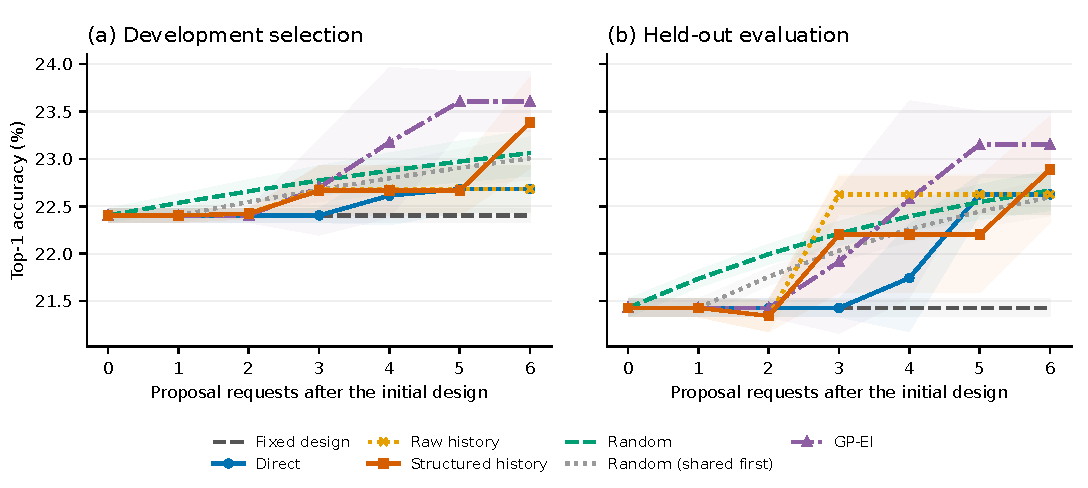
\includegraphics[width=\linewidth]{figures/fbhk_followup_20261109/history_prefix_dev_test.pdf}
\caption{Development selection and held-out prediction across the complete six-request study. Lines are means across three paired seeds and shading is sample standard deviation. Random curves integrate development-selected single-model outcomes at each budget, rather than depicting one random trajectory. The fixed reference has received its full 20-round fit. Held-out trajectories evaluate the development-selected model at each prefix, not the best model according to test scores.}
\label{fig:fbhk-prefix}
\end{figure}

\subsection*{E.7 Sensitivity to the single participating laboratory}
To examine whether laboratory 0 represents independent laboratories generally, we additionally train the fixed D00 design separately on every laboratory, 0--9, for proteomics, VCC, Norman and Tahoe. Each fit uses seed 42, 100 rounds, only that laboratory's training data and only its development panel for checkpoint selection. All 40 models, including laboratory 0, are newly fitted under the same CPU runtime and sealed before evaluation on the common task-specific test set. Saved predictions independently reproduce all 40 primary scores. The standard deviation here describes variation across laboratory identities at one seed, not training-seed variation or a collaborative model.

\begin{table}[t]
\centering
\small
\caption{Fixed-design sensitivity to the identity of the single participating laboratory. Each of ten laboratories independently fits D00 for 100 rounds and selects a checkpoint on its own development panel (seed 42). All 40 fits are fresh CPU runs under the same training equations; the SD and range describe laboratory identities, not training seeds. This diagnostic does not rerun research controllers.}
\label{tab:fbhk-lab-identity}
\begin{tabular}{lrrr}
\toprule
Endpoint & Lab 0 & Single-lab mean $\pm$ SD & Range \\
\midrule
Proteomics AP & 24.01 & $28.69 \pm 6.44$ & 14.69--37.34 \\
VCC Top-1 & 29.42 & $32.50 \pm 3.49$ & 26.96--39.76 \\
Norman Top-1 & 25.56 & $17.67 \pm 5.84$ & 4.37--25.56 \\
Tahoe Top-1 & 19.40 & $19.70 \pm 4.66$ & 13.43--26.87 \\
\bottomrule
\end{tabular}
\end{table}


Laboratory 0 is below the independent-laboratory mean for proteomics and VCC, close to it for Tahoe, and the highest-scoring laboratory for Norman. Thus its representativeness is task-dependent. These results supplement, rather than replace, the original three-seed GPU workflow scores. They evaluate fixed-model identity sensitivity, not a rotation of every search controller across laboratories. DTI is not included: its present preprocessing uses a training dictionary constructed from laboratory 0, so an isolated-laboratory rotation would also require a laboratory-specific dictionary and a separately registered initialization protocol. The same-ten-laboratory search controls in E.1--E.2 remain the direct comparison of search methods at fixed access.

\clearpage
\subsection*{E.8 Restoring target-panel feedback and auditing selection stability}
We version the source-defined cell and protein adapters, the outer target-evaluator reduction and the feedback projection together. Each recorded panel retains its identifier, primary score and loss. The payload distinguishes four training laboratories, ten target development panels and one evaluation worker; its worst-panel score and descriptive panel SD are computed from the recorded vector. The primary/loss selection key is unchanged. Raw and structured cards receive identical observed facts, including panel vectors at every recorded evaluation in new fits; direct receives no outcome scores. Missing vectors at unsaved intermediate checkpoints of old fits remain unavailable.

Before new development inference, we freeze both tasks, all twelve designs and seeds 61--63, then reconstruct the original 72 selected checkpoints and 720 labelled panel scores. Primary and loss reproduce exactly, while the true worst-panel score differs from the mean for all 72 checkpoints. Eight fresh CPU canary fits pair the original and repaired implementations on D00/D07, both tasks and seed 61 for ten rounds. Each pair has identical training losses, development primary/loss, selected round, selected weights and final training state. These are engineering checks, not additional full-budget search repetitions.

\begin{table}[htbp]
\centering
\small
\caption{Development-only audit after restoring target-panel feedback. Each row reconstructs all twelve saved best checkpoints. Gap is the mean across designs of primary minus the true worst-panel score, in percentage points. A/B are fixed even/odd panel subsets. The last column counts five-panel proposal subsets selecting the same design as all ten panels, out of 252. Complement scores reuse checkpoints already selected on all ten panels; they are descriptive, not independent confirmation.}
\label{tab:panel-feedback-audit}
\begin{tabular}{llrrrr}
\toprule
Task & Seed & Mean--worst gap & A gain & B gain & Winner agreement \\
\midrule
Cell & 61 & 20.13 & +17.13 & -2.68 & 102/252 \\
Cell & 62 & 19.77 & +13.58 & -8.54 & 77/252 \\
Cell & 63 & 19.67 & +13.18 & +13.19 & 166/252 \\
Protein & 61 & 54.63 & +0.00 & +0.00 & 43/252 \\
Protein & 62 & 53.93 & +0.00 & +0.00 & 16/252 \\
Protein & 63 & 55.20 & +1.67 & +0.00 & 72/252 \\
\bottomrule
\end{tabular}
\end{table}


We also predefine even-indexed panels for proposal selection and odd-indexed panels for a complementary diagnostic, keeping the existing saved checkpoints. Cell seeds 61/62 improve the proposal subset by 17.13/13.58 points but decrease its complement by 2.68/8.54 points; seed 63 improves both. Across all 252 five-panel proposal subsets, the all-panel winner is retained in only 102/77/166 cell cases and 43/16/72 protein cases. Exact primary ties use lower loss, so design disagreement need not imply a large primary-score difference. These subsets overlap and are not independent repetitions. Moreover, the checkpoints were originally selected on all ten panels, so complementary scores are descriptive rather than independent confirmation. The repair establishes faithful feedback transport; its effect on history-guided search, selection under a new protocol and generalization across new biological partitions remain untested.

\clearpage
\subsection*{E.9 Wider recipe choices at matched access and candidate budgets}
We examine whether the limited design library restricts model development on DTI and observed-response proteomics. A development-only capacity pilot fits 108 classifiers on the old 64-dimensional protein representation and two DTI configurations; its protein AP range is less than 0.2 development points. We retain these 110 fits as pilot costs and expand the protein input/model freedom before any new test evaluation. The formal study then trains all 36 recipes at seeds 71--73 on both tasks: 216 new fits shared by all search policies.

\paragraph{Models, recipes and development selection.}
Every policy starts from the same original fixed-default seed42 predictor per task. DTI freezes the fitted TAPB encoder and adapts its per-confounder classifier while retaining the original confounder-prior probability mixture. Protein either updates the complete original observed-response Conv1d/MLP head, or freezes it and adds a residual from the original 12,390 protein-response and Morgan-fingerprint inputs. These are warm-start studies, not replacements for the original end-to-end scores. The new seeds vary subsequent training and proposal generation, conditional on one common historical starting model; they are not three independent backbone fits.

The full recipe product combines learning rate $\{10^{-5},10^{-4},10^{-3}\}$, original-head fitting or a zero-output-initialized 32/128-wide residual, BCE or BCE plus 0.1 times within-batch positive--negative softplus ranking loss, and constant or cosine learning-rate schedules. The cosine schedule ends at 0.1 of its initial rate. Every fit completes 20 full-client rounds with AdamW reset locally each round, weight decay 0.001, gradient clipping at one and sample-weighted aggregation. Batch sizes are 256 for DTI and 64 for protein. Checkpoints at rounds 2/5/10/20 are selected by pooled development AUROC/AP, then lower pooled BCE and earlier round. This pooled selection differs from the original equal-panel protocol; all methods change together. Ten-panel diagnostics remain available, with undefined one-class metrics marked explicitly.

\paragraph{Matched proposers and conventional controls.}
Qwen2.5-7B and the Luna service each make six requests after a fitted D00, with one real first proposal shared across direct/raw/structured modes. All modes use the same recipe library, initialization, checkpoint rule, two-attempt limit and failure charges. Raw/structured receive the same queried facts, including all recorded panel trajectories. A reversible panel-table encoding prevents history truncation; every request checks exact reconstruction of its original card. Earlier interrupted controller runs remain engineering records. The Luna transport accepts only a completed text turn with recorded usage and no tool actions. Its generation seed and output-token cap cannot be enforced, and CLI context overhead is included in its token counts.

Random search exactly integrates all $\binom{35}{6}=1{,}623{,}160$ subsets and returns the expectation of a development-selected single predictor. These subsets are not independent training repetitions or prediction ensembles. We retain GP--EI with the original offset $\xi=.01$ and add $\xi=0$ as a stronger small-score-scale control, both at six requests. Shared-first and realized-fit-count random sensitivities are retained. Both proposer comparisons reuse the same control fits; repeated control values are not additional replications.

\paragraph{Outcomes and scope.}
Luna structured history reaches DTI AUROC 94.368 versus random's 94.316, a $+0.053$-point difference with paired conditional 95\% interval [0.031, 0.077] and gains in all three runs. Direct and raw history select the same DTI predictors. On protein, direct reaches 39.017 AP versus random's 38.655, while structured/raw history reaches 38.572. The prespecified structured-minus-random protein contrast is $-0.083$ points, with interval [$-2.025$, 2.234]; Qwen's is $-0.040$ [$-1.616$, 1.579]. Protein direct and the original GP--EI select identical final predictors in each seed. Thus the expanded workflow supplies models above random on both tasks, but the primary history comparison does not win both. This result does not establish an advantage from structured history over raw history or conventional search.

\clearpage
\begin{table}[htbp]
\centering\footnotesize
\setlength{\tabcolsep}{3pt}
\caption{Expanded-recipe comparison on DTI and proteomics. Each model uses the same 36 designs, ten training laboratories, six requests and 20 rounds per valid fit. Scores are means $\pm$ sample SD over three new head-training/controller runs, conditional on one shared seed42 starting predictor per task. DTI freezes the prior TAPB encoder; protein refits the complete observed-response head or a residual from all original inputs. Both proposer models and both GP offsets are retained. Bold marks the best means, including ties, not significance. These retrospective warm-start studies are separate from the original end-to-end scores.}
\label{tab:expanded-recipe-results}
\begin{tabular}{lrrrr}
\toprule
 & \multicolumn{2}{c}{Qwen2.5-7B} & \multicolumn{2}{c}{Luna service} \\
Policy & DTI AUROC & Protein AP & DTI AUROC & Protein AP \\
\midrule
Fully fitted D00 & $94.271 \pm 0.000$ & $37.109 \pm 0.000$ & $94.271 \pm 0.000$ & $37.109 \pm 0.000$ \\
Direct & $94.334 \pm 0.054$ & $38.244 \pm 0.465$ & $\mathbf{94.368 \pm 0.006}$ & $\mathbf{39.017 \pm 0.659}$ \\
Raw history & $\mathbf{94.368 \pm 0.006}$ & $38.533 \pm 0.886$ & $\mathbf{94.368 \pm 0.006}$ & $38.572 \pm 0.558$ \\
Structured history & $94.351 \pm 0.036$ & $38.616 \pm 0.826$ & $\mathbf{94.368 \pm 0.006}$ & $38.572 \pm 0.558$ \\
Random expectation & $94.316 \pm 0.007$ & $38.655 \pm 0.278$ & $94.316 \pm 0.007$ & $38.655 \pm 0.278$ \\
GP--EI ($\xi=.01$) & $94.290 \pm 0.029$ & $\mathbf{39.017 \pm 0.659}$ & $94.290 \pm 0.029$ & $\mathbf{39.017 \pm 0.659}$ \\
GP--EI ($\xi=0$) & $94.336 \pm 0.056$ & $37.975 \pm 0.837$ & $94.336 \pm 0.056$ & $37.975 \pm 0.837$ \\
\midrule
\multicolumn{5}{l}{\textit{Structured minus random; percentage points and conditional 95\% intervals}} \\
Proposer & DTI $\Delta$ & DTI interval & Protein $\Delta$ & Protein interval \\
Qwen & $+0.035$ & $[0.018, 0.054]$ & $-0.040$ & $[-1.616, 1.579]$ \\
Luna & $+0.053$ & $[0.031, 0.077]$ & $-0.083$ & $[-2.025, 2.234]$ \\
\bottomrule
\end{tabular}
\end{table}


All twelve task/seed/proposer selections are sealed before this study's test evaluation; saved predictions independently reproduce all 216 scores. Intervals use 2,000 paired bootstrap draws over DTI rows or protein compounds, shared across methods and seeds. They describe fixed-predictor test-sample uncertainty, not additional controller/backbone runs. The tests were exposed previously: this retrospective follow-up provides no new biological-split evidence. The separate cell benchmark in E.6 adds no new recipe-study result.

\begin{table}[htbp]
\centering\small
\caption{Actual candidate-cache construction and logical search budgets. Each task has 108 new fits. A fully valid six-request search uses seven fits. Different heads have different parameter counts and FLOPs; optimizer steps and example exposures are matched. Historical initial-predictor fitting, feature extraction, the 110-fit development pilot and interrupted engineering controller runs are reported separately in the provenance.}
\label{tab:expanded-recipe-cost}
\begin{tabular}{lrrrr}
\toprule
Task & Fits & Fit seconds & Steps/search & Exposures/search \\
\midrule
DTI & 108 & 1714.7 & 28,000 & 7,020,860 \\
Protein & 108 & 115.6 & 1,400 & 54,040 \\
\bottomrule
\end{tabular}
\end{table}


All-valid searches use seven complete fits and 140 full-client rounds: 28,000 optimizer steps/7,020,860 examples for DTI and 1,400/54,040 for protein. Different heads still have different FLOPs and runtime. Luna completes every logical slot; Qwen failures remain charged, with lower realized-fit random controls provided separately. The formal proposer runs use 182 Qwen and 101 Luna physical completions, including repairs. Common historical fitting, shared feature extraction, the pilot and interrupted engineering calls are additional costs, separate from each search's logical budget.
